\chapter{Descriptive overview of Edit Filters on the English Wikipedia}
\label{chap:overview-en-wiki}

The purpose of this chapter (syn?) is to explore the edit filters on the Englisch Wikipedia.
We want to gather a understanding of what types of tasks these filters take over,
and, as far as feasible, trace how these tasks have evolved over time.

%TODO describe what each section is about
The data upon which the analysis is based is described in section~\ref{sec:overview-data}
and the methods we use–in chapter 3.
Section~\ref{sec:patterns} explores (syn) some patterns in the edit filters' usage and..
And we look into the manual classification of EN Wikipedia's edit filters I've undertaken in an attempt to understand what is it that they actually filter in section~\ref{sec:manual-classification}.


\section{Data}
\label{sec:overview-data}

The main part of the present analysis rests upon/is based upon/is grounded in/foundations lie the \emph{abuse\_filter} table from \emph{enwiki\_p}(the database which stores data for the EN Wikipedia), or more specifically a snapshot thereof which was downloaded on January 6th, 2019 via quarry, a web-based service offered by Wikimedia for running SQL queries against their public databases~\footnote{\url{https://quarry.wmflabs.org/}}.
The complete dataset can be found in the repository for the present paper~\cite{github}. % TODO add a more specific link

This table, along with \emph{abuse\_filter\_actions}, \emph{abuse\_filter\_log}, and \emph{abuse\_filter\_history}, are created and used by the AbuseFilter MediaWiki extension~\cite{gerrit-abusefilter-tables}, as discussed in section~\ref{sec:mediawiki-ext}.
Selected queries have been run via quarry against the \emph{abuse\_filter\_log} table as well.
Unfortunately, the \emph{abuse\_filter\_history} table which will be necessary for a complete historical analysis of the edit filters is currently not exposed to the public due to security/privacy concerns~\cite{phabricator}.
Therefore, the present work only touches upon historical trends in a qualitative fashion. %TODO how are these determined: API to abuse_filter_history; general stats from abuse_filter
or qualitatively shows patterns.
A comprehensive historical analysis is therefore (syn!) one of the possibilities/directions for future studies (syn).

%TODO maybe move to appendix; mention tables have been discussed in~\ref{sec:mediawiki-ext} and only quote here the one for abuse\_filter since we are using the data
A concise description of the tables has been offered in section~\ref{sec:mediawiki-ext} which discusses the AbuseFilter MediaWiki extension in more detail.
Here, only the schema of the \emph{abuse\_filter} table has been included (figure~\ref{fig:db-schemas-af}), since that is the data the present analysis is based upon.
For further reference, the schemas of all four tables can be viewed in figures~\ref{fig:app-db-schemas-af},~\ref{fig:app-db-schemas-afl},~\ref{fig:app-db-schemas-afh} and~\ref{fig:app-db-schemas-afa} in the appendix.

\begin{figure*}
\begin{verbatim}
abuse_filter
+--------------------+----------------+------+-----+---------+----------------+
| Field              | Type           | Null | Key | Default | Extra          |
+--------------------+----------------+------+-----+---------+----------------+
| af_id              | bigint(20)     | NO   | PRI | NULL    | auto_increment |
| af_pattern         | blob           | NO   |     | NULL    |                |
| af_user            | bigint(20)     | NO   | MUL | NULL    |                |
| af_user_text       | varbinary(255) | NO   |     | NULL    |                |
| af_timestamp       | binary(14)     | NO   |     | NULL    |                |
| af_enabled         | tinyint(1)     | NO   |     | 1       |                |
| af_comments        | blob           | YES  |     | NULL    |                |
| af_public_comments | tinyblob       | YES  |     | NULL    |                |
| af_hidden          | tinyint(1)     | NO   |     | 0       |                |
| af_hit_count       | bigint(20)     | NO   |     | 0       |                |
| af_throttled       | tinyint(1)     | NO   |     | 0       |                |
| af_deleted         | tinyint(1)     | NO   |     | 0       |                |
| af_actions         | varbinary(255) | NO   |     |         |                |
| af_global          | tinyint(1)     | NO   |     | 0       |                |
| af_group           | varbinary(64)  | NO   | MUL | default |                |
+--------------------+----------------+------+-----+---------+----------------+
\end{verbatim}
  \caption{abuse\_filter schema}~\label{fig:db-schemas-af}
\end{figure*}

\section{Descriptive statistics/Patterns}
\label{sec:patterns}

In this section, we explore some general patterns of the edit filters on Engish Wikipedia, or respectively the data from the \emph{abuse\_filter} table.
The scripts that generate the statistics discussed here, can be found in the jupyter notebook in the project's repository. %TODO add link after repository has been cleaned up

\subsection{Filter characteristics}
As of January 6th, 2019 there are $954$ filters in this table.
It should be noted, that if a filter gets deleted, merely a flag is set to indicate so, but no entries are removed from the database.
So, the above mentioned $954$ filters are all filters ever made up to this date.
This doesn't mean that it never changed what the filters are doing, since, as pointed out in chapter~\ref{}, edit filter managers can freely modify filter patterns, so at some point the filter could be doing one thing and in the next moment, it is filtering a completely different phenomenon.
This doesn't happen very often though.
$361$ of all filters are public, the remaining $593$–hidden.
$110$ of the public ones are active, $35$ are disabled, but not marked as deleted, and $216$ are flagged as deleted.
Out of the $593$ hidden filters $91$ are active, $118$ are disabled (not deleted), and $384$ are deleted.
The relative proportion of these groups to each other can be viewed on figure~\ref{fig:general-stats}.

\begin{figure}
\centering
  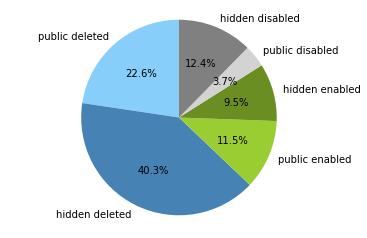
\includegraphics[width=0.9\columnwidth]{pics/general_stats.png}
  \caption{EN Wikipedia edit filters: hidden, disabled and deleted filters}~\label{fig:general-stats}
\end{figure}

%TODO decide whether to keep data of the sort; it's not very accurate (since hidden filters are missing), there is no interesting tendency and I don't have any particular commentary on it.
Table ... show how many new filters have been introduced over the years.
2009: ~280 ; 1~27x (hidden, so we don't know)
2010: ~100 ; 280 (6.1.2010)- smth between 379 (28.12.2010) and 384 (10.2.2011)
2011: ~70  ; ~380 - 44x (440 is Nov 2011, 458 is April 2012)
2012: ~70  ; ~450 - 51x (514 is Dec 2012, 520 is Jan 2013)
2013: ~80  ; ~520 - 59x (593 is 3.10.2013, 602 is 15.1.2014)
2014: ~55  ; ~600 - 65x (650 is 16.12.2014, 655 is 19.1.2015)
2015: ~90  ; ~655 - ~745 (744 is 28.12.2015, 747 is 7.1.2016)
2016: ~75  ; ~745 - 81x (812 is 3.12.2016, 828 is 19.1.2017)
2017: ~75  ; ~820 - 89x (894 is 23.12.2018, 897 is 8.1.2018)
2018: ~55  ; ~895 - (949 is 16.12.2018)


Another parameter we could observe are the currently configured filter actions for each filter.
Figure~\ref{fig:all-filters-actions} depicts action per filter (note this includes all filters, also deleted ones and that some filters have multiple actions enabled).
And figures~\ref{fig:active-public-actions} and~\ref{fig:active-hidden-actions} the actions of all enabled public and hidden filters respectively.
It is noticeable that the most common action for the enabled hidden filters is ``disallow'' whereas most enabled public filters are set to ``tag'' or ``tag,warn''.
This coincides/is congruent with the community claim that hidden filters target particularly perstistent vandalism, which is best outright disallowed.
Most public filters on the other hand still assume good faith from the editors and try to dissuade them from engaging in disruptive behaviour by using warnings or just tag conspicious behaviour for further investigation.

\begin{figure}
\centering
  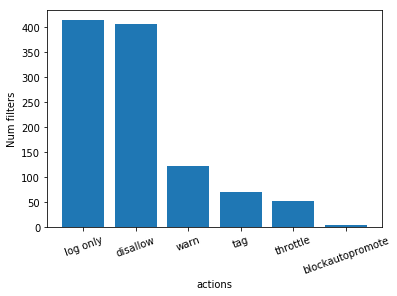
\includegraphics[width=0.9\columnwidth]{pics/all-filters-actions.png}
  \caption{EN Wikipedia edit filters: Filters actions for all filters}~\label{fig:all-filters-actions}
\end{figure}

\begin{figure}
\centering
  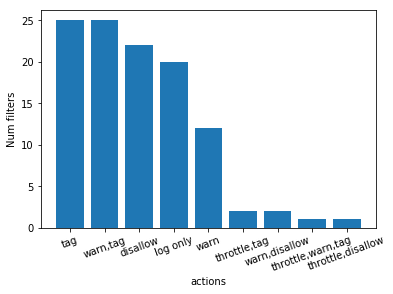
\includegraphics[width=0.9\columnwidth]{pics/active-public-filters-actions.png}
  \caption{EN Wikipedia edit filters: Filters actions for enabled public filters}~\label{fig:active-public-actions}
\end{figure}

\begin{figure}
\centering
  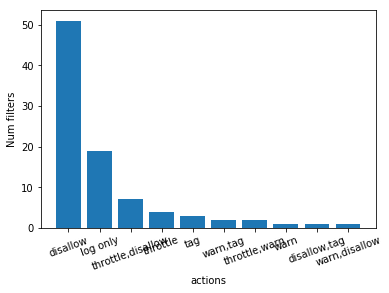
\includegraphics[width=0.9\columnwidth]{pics/active-hidden-filters-actions.png}
  \caption{EN Wikipedia edit filters: Filters actions for enabled hidden filters}~\label{fig:active-hidden-actions}
\end{figure}


\subsection{Filter makers}

Here, a few characteristics of the edit filter managers group are discussed.
As mentioned in section~\ref{}, EN Wikipedia has 154 edit filter managers as of (date).
The group is as discussed (syn!) quite small.
(However, for comparison there are only 4 users in the edit filter managers group on the Catalan Wikipedia and the role does not exist at all on the German, Spanish and Russian ones which leads to the assumption that for these languages all administrators have the \emph{abusefilter\_modify} permission.)

The edit filter managers group is quite stable, with only 4 users who have become an edit filter manager since November 2016 (according to the discusssion archives of the edit filter noticeboard where the permission is requested).
Since the edit filter helper group has been created in September 2017, only 11 users have been granted the corresponding permissions and only one of them has been subsequently ``promoted'' to become an edit filter manager.
(Interestingly, currently (July 2019) there are 19 people in the edit filter helpers group, so apparently some of them have received the right although no records are there on the noticeboard??)

Moreover, quite some of the 154 edit filter managers on English Wikipedia have a kind of ``not active at the moment'' banner on their user page, which leads to the conclusion that the edit filter managers group is aging.

% Has it been the same people from the very beginning?

% What type of work do the different managers take over?
There are a couple of very active managers who seem to keep an overview over all filters and do maintenance work on them e.g. updating conditions to optimise evaluation or updating (syn!) deprecated variable names upon updates (syn!) of the extension's code.

Further interesting questions come to mind such as whether there are edit filter managers who specialise in creating different types of edit filters (compare manual classification).
However, in order to be able to answer this, an access to the whole \emph{abuse\_filter\_history} table is needed, so this remains a question (syn!) for future inquiry.



\subsection{Filter activity}

Thanks to quarry, we have all the filters that were triggered from the filter log per year, from 2009 (when filters were first introduced/the MediaWiki extension was enabled) till end of 2018, with their corresponding number of times being triggered:
Table~\ref{tab:active-filters-count} summarises the numbers of distinct filters that got triggered over the years.
So, the number of distinct filters that have been triggered over the years varies between $154$ in year 2014 and $254$ in 2018.
The explanation for this not particularly wide range of active filters lies probably in the so-called condition limit.
According to the edit filters' documentation~\cite{Wikipedia:EditFilterDocumentation}, the condition limit is a hard-coded treshold of total available conditions that can be evaluated by all active filters.
Currently, it is set to $1,000$.
The motivation for the condition limit is to avoid performance issues since every incoming edit is checked against all currently active filters which means that the more filters are active the longer the checks take.
However, the page also warns that counting conditions is not the ideal metric of filter performance, since there are simple comparisons that take significantly less time than a check against the \emph{all\_links} variable for example (which needs to query the database)~\cite{Wikipedia:EditFilterDocumentation}.

\begin{table}
  \centering
  \begin{tabular}{l r }
    % \toprule
    Year & Num of distinct filters \\
    \hline
    2009 & 220 \\
    2010 & 163 \\
    2011 & 161 \\
    2012 & 170 \\
    2013 & 178 \\
    2014 & 154 \\
    2015 & 200 \\
    2016 & 204 \\
    2017 & 231 \\
    2018 & 254 \\
    % \bottomrule
  \end{tabular}
  \caption{Count of distinct filters that got triggered each year}~\label{tab:active-filters-count}
\end{table}

The ten most active filters of all times (with number of hits and public description) are displayed in table~\ref{tab:most-active-actions}.
For a more detailed reference, the ten most active filters of each year are listed in the appendix. %TODO are there some historical trends we can read out of it?
and, of course, the whole \emph{abuse\_filter} table snapshot can be consulted in the repository~\cite{github}.

Already, a couple of patterns draw attention when we look at the most active (syn!) filters:
They seem to catch a combination of possibly good faith edits which were none the less unconstructive (such as removing references, section blanking or large deletions)
and what the community has come to call ``silly vandalism''~\cite{Wikipedia:VandalismTypes}: repeating characters and inserting profanities.
Interestingly, that's not what the developers of the extension believed it was going to be good for:
``It is not, as some seem to believe, intended to block profanity in articles (that would be extraordinarily dim), nor even to revert page-blankings, '' claimed its core developer on July 9th 2008~\cite{Wikipedia:EditFilterTalkArchive1}.
Rather, among the 10 most active filters, it is filter 527 ``T34234: log/throttle possible sleeper account creations'' which seems to target what most closely resembles the intended aim of the edit filter extension. %TODO explain again what the intended aim was

Another assumption that proved to be wrong/didn't quite carry into effect was that ``filters in this extension would be triggered fewer times than once every few hours''.
As a matter of fact, a quick glance at the AbuseLog~\footnote{\url{https://en.wikipedia.org/wiki/Special:AbuseLog}} confirms that there are often multiple filter hits per minute.

\begin{table*}
  \centering
    \begin{tabular}{r r p{8cm} p{2cm} }
    % \toprule
        Filter ID & Hitcount & Publicly available description & Actions \\
    \hline
       61 & 1,611,956 & new user removing references & tag \\
      135 & 1,371,361 & repeating characters & tag, warn \\
      527 & 1,241,576 & T34234: log/throttle possible sleeper account creations (hidden filter) & throttle \\
      384 & 1,159,239 & addition of bad words or other vandalism & disallow \\
      172 & 935,925 & section blanking & tag \\
       30 & 840,871 & large deletion from article by new editors & tag, warn \\
      633 & 808,716 & possible canned edit summary & tag \\
      636 & 726,764 & unexplained removal of sourced content & warn \\
        3 & 700,522 & new user blanking articles & tag, warn \\
      650 & 695,601 & creation of a new article without any categories & (log only) \\
  \end{tabular}
  \caption{What do most active filters do?}~\label{tab:most-active-actions}
\end{table*}

%TODO compare with table and with most active filters per year: is it old or new filters that get triggered most often? (I'd say it's a mixture of both and we can now actually answer this question with the history API, it shows us when a filter was first created)

We can follow/track/backtrack the number of filter hits over the years (syn) on figure~\ref{fig:filter-hits}.
There is a dip in the number of hits in late 2014 and quite a surge in the beginnings of 2016.
Here is the explanation to that:
%TODO discuss peak! (and overall pattern)
\begin{comment}
Looking at january 2016:

till now it comes to attention that a lot of accounts named something resembling <FirstnameLastname4RandomLetters> were trying to create an account  (while logged in?) (or maybe it was just that the creation of these particular accounts itself was denied); this triggers filter 527 ("T34234: log/throttle possible sleeper account creations
")
There are in the meantime over 5 pages of them, it is definitely happening automatically

TODO: download data; write script to identify actions that triggered the filters (accountcreations? edits?) and what pages were edited
Note: do hidden filters appear in this numbers and in the table? (They are definitely not displayed in the front end of the AbuseLog) -- they do.
\end{comment}

%TODO strectch plot so months are readable; darn. now it's too small on the pdf. Fix it! May be rotate to landscape?
\begin{figure}
\centering
  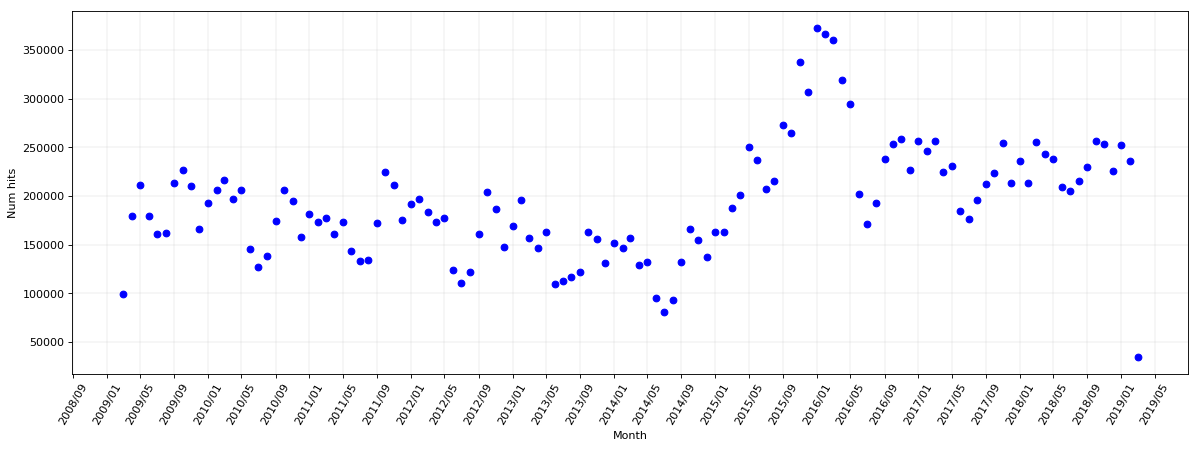
\includegraphics[width=0.9\columnwidth]{pics/filter-hits-zoomed.png}
  \caption{EN Wikipedia edit filters: Number of hits per month}~\label{fig:filter-hits}
\end{figure}


\begin{comment}
    \item how often were filters with different actions triggered? (afl\_actions) (over time) --> abuse\_filter\_log
    \item what types of users trigger the filters (IPs? registered?) : IPs: 16,489,266, logged in users: 6,984,897 (Stand 15.03.2019);
    \item on what articles filters get triggered most frequently (afl\_title)
    \item what types of user actions trigger filters most frequently? (afl\_action) (edit, delete, createaccount, move, upload, autocreateaccount, stashupload)
    \item in which namespaces get filters triggered most frequently?
    %TODO categorise filters according to which name spaces they apply to; pay special attention to edits in user/talks name spaces (may be indication of filtering harassment) -- check notebook
\end{comment}

\begin{comment}
    \item is it new filters that get triggered most frequently? or are there also very active old ones? -- we have the most active filters per year, where we can observe this. It's a mixture of older and newer filter IDs (they get an incremental ID, so it is somewhat obvious what's older and what's newer); is there a tendency to split and refine older filters?
\end{comment}

\section{Patterns in filters creation and usage}

The present section explores qualitatively/highlights patterns in the creation and usage of edit filters.
Unfortunately, no extensive quantitative analysis of these patterns was possible, since for it, an access to the \emph{abuse\_filter\_history} table is needed.
The table is currently not replicated via.. and no public dump is accessible via the toolserver. %TODO elaborate
This seems to have been the case in the past, however, due to security concerns the dumps were discontinued. %TODO cite phabricator
A short term solution to renew the public replicas was not possible, so the present chapter only shows some patterns (syn!) observed via manual browsing of different filters' history via the exposed API endpoint which allows querying the \emph{abuse\_filter\_history} table for public filters.

\subsection{Usage}

Following general patterns (syn!) of filter usage were observed:
There are filters that have been switched on for a while, then deactivated and never activated again.
Some of them had only been active very briefly before they were switched off and deleted.
There are a couple of different reasons for that:
The filter in question was only testing a pattern which was eventually merged in another filter (e.g.: ). 440 was merged in 345 (or was it a duplicate?)
The edit filter managers decided not to implement the filter, because edit filters were deemed an inappropriate tool to deal with the problem at hand (e.g. ...)308), 199 ('Unflagged Bots');
  ** switched off, bc filter was deemed inappropriate to deal with the issue at hand: 484 "Shutdown of ClueBot by non-admin user" (From the comments: " Just sysop-protect the page if you don't want non-admins messing with it. --Reaper 2012-09-06")
or decides to not implement the thing (that way); 290 (disabled, since relevant pages were protected);
or, because there were hardly any hits, so there wasn't really a problem at all ( 304, 67, 122, 401 ("Red hair" vandalism)). %result of editors implementing a filter "just to see if it catches anything"?
There are also cases in which filter managers implement a filter targeting the same phenomenon in parallel and without knowing of each other.
These duplicate cases (syn!) are also merged eventually, or alternatively all but one of them are switched off: 891 and 893
Sometimes, vandalism trends are only temporary and after a period of activity, the filters become stale.
This is also a reason for filters to be eventually powered off in order to save conditions from the condition limit.
Examples thereof are:302 (switched off on the grounds of insufficient activity),81 (bad charts)
 211 ("Disable, appears to be inactive (log only filter). If you are using this filter, please let me know, and I'll reenable it -Prodego"); 20 ("A waste of processor time, deleted -Prodego"); 663?
There are also filters that were switched off because they weren't doing what they were supposed to and only generated a big amount of false positives: (false positives is a plausible option here): 394,  14 (disabled in couple of hours)

\begin{comment}
%TODO This is a duplicate of a paragraph in 4.5.1. Does it fit better here?
% this actually fits also in the patterns of new filters in chap.5; these are the filters introduced for couple of days/hours, then switched off to never be enabled again
Edit filter managers often introduce filters based on some phenomena they have observed caught by other filters, other algorithmic quality control mechanisms or general experience.
As all newly implemented filters, these are initially enabled in logging only mode until enough log entries are generated to evaluate whether the incident is severe and frequent enough to need a filter.
\end{comment}

Then, there are filters switched on for a while, deactivated for a while and activated again.
Sometimes because a pattern of vandalism is re-occuring, and sometimes–in order to fix technical issues with the filters: 61, 98 (was deactivated briefly since an editor found the "warn" action unfounded; re-enabled to tag), 148 ("20160213 - disabled - possible technical issue - see edit filter noticeboard - xaosflux")

Another group constitute enabled filters that have never been switched off since their introduction.
  11 (verify), 79 (with brief periods of being disabled for couple of minutes/hours, probably in order to update the pattern), 164, 642 (if we ignore the 2min period it was disabled on 13.4.2018), 733 (2.11.2015-present), 29 (18.3.2009-present), 30 (18.3.2009-present), 33 (18.3.2009-present), 39 (18.3.2009-present), 50 (18.3.2009-present), 59 (19.3.2009-present), 80 (22.3.2009-present)
There are also some filters that have always been enabled with the exception of brief periods of time when the filter was deactivated (and the activated again), probably in order to update the conditions: 79, 135 (there were couple of others in Shirik's list, go back and look);
There seems to be a tendency that all actions but logging (which cannot be switched off) are took out, when edit filter managers are updating the regex of the filter.

Oftentimes, when a hidden filter is marked as ``deleted'', it is made public. (examples!)

%TODO leave this here or move to filter characteristics?
It is not uncommon, that the action(s) a particular filter triggers change over time.
As of the guidelines for implementing new filters, every filter should be enabled in ``log only'' mode at its introduction.
After it has been deemed that the filter actually acts as desired, usually additional actions are switched on~\cite{Wikipedia:EditFilterInstructions}.
Sometimes, when a wave of particularly persistent vandalism arises, a filter is temporarily set to ``warn'' or ``disallow'' and the actions are removed again as soon as the filter is not tripped very frequently anymore. %TODO examples?

\subsection{What do filters target}%: general behaviour vs edits by single users

Most of the public filters target general disruptive behavious (e.g.?).
There are however some which target particular users or particular pages.
Arguably, (see guidelines) an edit filter may not be the ideal mechanism for this latter purpose, since every incoming edit is checked against all active filters.
Historically, filters have been introduced to track some specific sort of behaviour which was however neither malicious nor disruptive.
This contradicts/defies/fails the purpose of the mechanism and thus such filters have been (quite swiftly) disabled.
Some filters target (syn!) insults in general, and there are such which target (syn!) specifically insults aimed at particular persons (often edit filter managers).

\begin{comment}
  ** there are quite some filters targeting particular users: 290 (targets an IP range), 177 ('User:Television Radio'), 663 ('Techno genre warrior
', targets specific IP ranges)
  ** there are also some targetting particular pages (verify!), although this clashed with the guidelines: 264 "Specific-page vandalism" (it's hidden though, so we don't know what exactly it's doing); 401 ("Red hair" vandalism); there's smth with the main page; 715 "IP notification on RFP/C"
  ** there are also filters such as 199 (Unflagged bots) which were implemented in order to track something which was not quite malicious or abusive and were thus deemed inappropriate use of filters by the community and consequently (quite swiftly) deleted
  ** some target insults in general and some contain regexes containing very specifically insults directed towards edit filter managers (see filter 12)
\end{comment}

\subsection{How do filters emerge?}
  ** an older filter is split? 79 was split out of 61, apparently; 285 is split between "380, 384, 614 and others"; 174 is split from 29
  ** several older filters are merged?
  ** or functionality of an older filter is took and extended in a newer one (479->631); (82->278); (358->633);
  ** new condition(s) are tested and then merged into existing filter : stuff from 292 was merged to 135 (https://en.wikipedia.org/wiki/Special:AbuseFilter/history/135/diff/prev/4408 , also from 366; following the comments from https://en.wikipedia.org/wiki/Special:AbuseFilter/292 it was not conceived as a test filter though, but it was rather merged in 135 post-factum to save conditions); 440 was merged into 345; apparently 912 was merged into 11 (but 11 still looks like checking for "they suck" only^^); in 460: "Merging from 461, 472, 473, 474, and 475. --Reaper 2012-08-17"
  ** an incident caught repeatedly by a filter motivates the creation of a dedicated filter (994)
  ** filter is shut down, because editors notice there are 2 (or more filters) that do nearly identical checks: 344 shut down because of 3

  ** "in addition to filter 148, let's see what we get - Cen" (https://en.wikipedia.org/wiki/Special:AbuseFilter/188) // this illustrates the point that edit filter managers do introduce stuff they feel like introducing just to see if it catches something

\section{Public and Hidden Filters}

The first noticeable typology is along the line public/private filters.

It draws attention that currently nearly $2/3$ of all edit filters are not viewable by the general public (compare figure~\ref{fig:general-stats}).
Unfortunately, without the full \emph{abuse\_filter\_history} table we cannot know how this ration has developed historically.
However, the numbers fit the assertion of the extension's core developer according to whom edit filters target particularly determined vandals.

Although the initial plan was to make all filters hidden, the community discussions rebutted that so a guideline was drafted calling for
hiding filters ``only where necessary, such as in long-term abuse cases where the targeted user(s) could review a public filter and use that knowledge to circumvent it.''~\cite{Wikipedia:EditFilter}.
Further, caution in filter naming is suggested for hidden filters and editors are encouraged to give such filters just simple description of the overall disruptive behaviour rather than naming a specific user that is causing the disruptions.
(The later is not always complied with, there are indeed filters named after the accounts causing a disruption.)

Only edit filter editors (who have the \emph{abusefilter-modify} permission) and editors with the \emph{abusefilter-view-private} permission can view hidden filters.
The later is given to edit filter helpers - editors interested in helping with edit filters who still do not meet certain criteria in order to be granted the full \emph{abusefilter-modify} permission, editors working with edit filters on other wikis interested in learning from the filter system on English Wikipedia, and Sockpuppet investigation clerks~\cite{Wikipedia:EditFilterHelper}.
As of March 17, 2019, there are 16 edit filter helpers on EN Wikipedia~\footnote{\url{https://en.wikipedia.org/wiki/Special:ListUsers/abusefilter-helper}}.
Also, all administrators are able to view hidden filters.

There is also a designated mailing list for discussing these: wikipedia-en-editfilters@lists.wikimedia.org.
It is specifically indicated that this is the communication channel to be used when dealing with harassment (by means of edit filters)~\cite{Wikipedia:EditFilter}.
It is signaled, that the mailing list is meant for sensitive cases only and all general discussions should be held on-wiki~\cite{Wikipedia:EditFilter}.

%TODO decide whether to include this here or move back to actions
  ** there's a tendency of editors to hide filters just for the heck of it (at least there are never clear reasons given), which is then reverted by other editors with the comment that it is not needed: 148, 225 (consesus that general vandalism filters should be public \url{[Special:Permalink/784131724#Privacy of general vandalism filters]}), 260 (similar to 225), 285 (same), 12 (same), 39 (unhidden with the comment "made filter public again - these edits are generally made by really unsophisticated editors who barely know how to edit a page. --zzuuzz")


\section{Types of edit filters: Manual Classification}
\label{sec:manual-classification}

The aim of this section is to get a better understanding of what exactly it is that edit filters are filtering.
Based on grounded theory methodology presented in chapter~\ref{chap:methods}, I applied emergent coding to all filters, scrutinising their patterns, comments and actions.
%TODO Comment on exact process of coding (check with coding book, I think a lot is explained there already)

Three big clusters of filters were identified, namely ``vandalism'', ``good faith'' and ``maintenance''. %TODO define what each of them are

It was not always a straightforward decision to determine what type of edits a certain filter is targeting.
This was of course, particularly challenging for private filters where only the public comment (name) of the filter was there to guide the coding.
On the other hand, guidelines state up-front that filters should be hidden only in cases of particularly persistent vandalism, in so far it is probably safe to establish that all hidden filters target some type of vandalism.
However, the classification was difficult for public filters as well, since oftentimes what makes the difference between a good-faith and a vandalism edit is not the content of the edit but the intention of the editor.
While there are cases of juvenile vandalism (putting random swear words in articles) or characters repetiton vandalism which are pretty obvious, that is not the case for sections or articles blanking for example.
For these, from the edit alone there is no way of knowing whether the deletion was malicious or the editor conducting it just wasn't familiar with say the correct procedure for moving an article.

%TODO compare with code book and kick the paragraph out
In such ambiguous cases, we can be guided by the action the filter triggers (if it is ``disallow'' the filter is most probably targeting vandalism).
At the end, we labeled most ambiguous cases with both ``vandalism'' and ``good faith''.


%TODO include here a diagram with overview of the categories distribution

In the subsections that follow the salient properties of each manually labeled category are discussed.

\subsection{Vandalism}

The vast majority of edit filters on EN Wikipedia could be said to target (different forms of) vandalism, i.e. maliciously intended disruptive editing.
Examples thereof are filters for juvenile types of vandalism (inserting swear or obscene words or nonsence sequences of characters into articles), for hoaxing (inserting obvious or less obvious false information in articles) or for template vandalism (modifying a template in a disruptive way which is quite severe, since templates are displayed on various pages).
A more elaborate subclassification was conducted; all codes belonging to the vandalism cluster together with definition and examples can be consulted in the code book attached in the appendix~\ref{}.

Some vandalism types seem to be more severe than others (sock puppetry or persistant long term vandals).
It's mostly in these cases that the implemented filters are hidden.

%TODO where is the best place for this? I've got the feeling it's explained somewhere already and here it's quite late
\begin{comment}
This means, only edit filter editors can view the exact filter pattern or the comments of these.
Although this clashes with the overall *transparency* of the project (is there a guideline subscribing to this value? couldn't find a specific mention), the reasoning here is that otherwise, persistent vandals will be able to check for the pattern of the filter targetting their edits and just find a new way around it~\cite{Wikipedia:EditFilter}. %TODO compare with https://en.wikipedia.org/w/index.php?title=Wikipedia:About&oldid=891256910 about transparency as a value

The current state is also an "improvement" compared to the initially proposed visibility level of edit filters.
In the initial version of the EditFilters Page (https://en.wikipedia.org/w/index.php?title=Wikipedia:Edit_filter&oldid=221158142) Andrew Garrett (User:Werdna), the author of the AbuseFilter MediaWiki extension, was suggesting that all filters should be private and only a group of previously approved users should be able to view them.
    (This was met by the community with a strong resistence, especially since at the time one of the most discussed features was the ability of filters to (temporarily) block users. Editors involved in the discussion felt strongly that no fully automated agent should be able to block human editors.)
\end{comment}

There are also private filters targetting personal attack or abuse cases.
Here, filters are private in order to protect the affected person(s)~\cite{Wikipedia:EditFilter}.
A dedicated subcluster of ``hardcore vandalism'' was defined (syn!) for these cases.

%TODO what to make out of this? It's kind of interesting but doesn't really serve any purpose..
\begin{comment}
motivations:
- seeking attention
- misusing the encyclopedia for own purposes (self-promotion, seo..)
- spreading wrong information
- defacing topics
\end{comment}

\begin{comment}
%TODO decide what to do with all of this. Probably just leave out
## Consequences of vandalism, vandalism management
https://en.wikipedia.org/wiki/Wikipedia:Vandalism
"Vandalism is prohibited. While editors are encouraged to warn and educate vandals, warnings are by no means a prerequisite for blocking a vandal (although administrators usually only block when multiple warnings have been issued). "

"Upon discovering vandalism, revert such edits, using the undo function or an anti-vandalism tool. Once the vandalism is undone, warn the vandalizing editor. Notify administrators at the vandalism noticeboard of editors who continue to vandalize after multiple warnings, and administrators should intervene to preserve content and prevent further disruption by blocking such editors. Users whose main or sole purpose is clearly vandalism may be blocked indefinitely without warning."

% TODO maybe keep this part, not exactly clear where
One of the strategies to spot vandalism is "Watching for edits tagged by the abuse filter. However, many tagged edits are legitimate, so they should not be blindly reverted. That is, do not revert without at least reading the edit." //mention of filters!

"Warn the vandal. Access the vandal's talk page and warn them. A simple note explaining the problem with their editing is sufficient. If desired, a series of warning templates exist to simplify the process of warning users, but these templates are not required. These templates include

    Level one: {{subst:uw-vandalism1}} This is a gentle caution regarding unconstructive edits; it encourages new editors to use a sandbox for test edits. This is the mildest warning.
    Level two: {{subst:uw-vandalism2}} This warning is also fairly mild, though it explicitly uses the word 'vandalism' and links to this Wikipedia policy.
    Level three: {{subst:uw-vandalism3}} This warning is sterner. It is the first to warn that further disruptive editing or vandalism may lead to a block.
    Level four: {{subst:uw-vandalism4}} This is the sharpest vandalism warning template, and indicates that any further disruptive editing may lead to a block without warning."
\end{comment}

\subsection{Disruptive Editing}

According to https://en.wikipedia.org/wiki/Wikipedia:Vandalism various behaviours are (highly) disruptive albeit not vandalism.
Filters targeting such behaviours (syn) were identified and grouped in the ``disruptive editing'' cluster. %TODO elaborate with code book

\begin{comment}
- boldly editing
- copyright violation
- disruptive editing or stubbornness --> edit warring
- edit summary omission
- editing tests by experimenting users: "Such edits, while prohibited, are treated differently from vandalism"
- harassment or personal attacks: "Personal attacks and harassment are not allowed. While some harassment is also vandalism, such as user page vandalism, or inserting a personal attack into an article, harassment in itself is not vandalism and should be handled differently."
- Incorrect wiki markup and style
- lack of understanding of the purpose of wikipedia: "editing it as if it were a different medium—such as a forum or blog—in a way that it appears as unproductive editing or borderline vandalism to experienced users."
- misinformation, accidental
- NPOV contraventions (Neutral point of view)
- nonsense, accidental: "sometimes honest editors may not have expressed themselves correctly (e.g. there may be an error in the syntax, particularly for Wikipedians who use English as a second language)."
- Policy and guideline pages, good-faith changes to: "If people misjudge consensus, it would not be considered vandalism;"
- Reversion or removal of unencyclopedic material, or of edits covered under the biographies of living persons policy: "Even factually correct material may not belong on Wikipedia, and removing such content when it is not in line with Wikipedia's standards is not vandalism."
- Deletion nominations: "Good-faith nominations of articles (or templates, non-article pages, etc) are not vandalism."
\end{comment}

Several of these behaviours could actually be conceived as **good faith** edits.
And, for several of them (as noted in the **good faith memo**), it is not immediately distinguishable whether it's a **good faith** or a **vandalism** edit.
Ultimately, the "only" difference between the two arises from the motivation/context of the edit.


\subsection{Good Faith}
\begin{comment}
# Good faith edits

*Good faith* is a term used by the Wikipedia community itself.
Most prominently in the phrase "Always assume good faith".

As I recently learned, apparently this guideline arose/took such a central position not from the very beginning of the existence of the collaborative encyclopedia.
It rather arose at a time when, after a significant growth in Wikipedia, it wasn't manageable to govern the project (and most importantly fight emergent vandalism which grew proportionally to the project's growth) manually anymore.
To counteract vandalism, a number of automated measures was applied.
These, however, had also unforseen negative consequences: they drove newcomers away~\cite{HalKitRied2011}(quote literature) (since their edits were often classified as "vandalism", because they were not familiar with guidelines / wiki syntax / etc.)
In an attempt to fix this issue, "Assume good faith" rose to a prominent position among Wikipedia's Guidelines.
(Specifically, the page was created on March 3rd, 2004 and was originally refering to good faith during edit wars.
An expansion of the page from December 29th 2004 starts refering to vandalism. https://en.wikipedia.org/w/index.php?title=Wikipedia:Assume_good_faith&oldid=8915036)

Today, in vandalism combating (?), there are guidelines that plead for caution and several escalation levels, before an editor is banned. (TODO: elaborate, maybe move to vandalism)
Users are urged to use the term "vandalism" carefully, since it tends to offend and drive people away.
("When editors are editing in good faith, mislabeling their edits as vandalism makes them less likely to respond to corrective advice or to engage collaboratively during a disagreement,"~\cite{Wikipedia:Vandalism})
Not all disruptive behaviour is vandalism, the guidelines suggest~\cite{Wikipedia:Vandalism}.

Examples of "good faith" edits that are non the less disruptive are not complying with Wiki syntax (mostly because of being unfamiliar with it), deleting a page instead of moving it, using improper redirects or publishing test changes; also because of being unaware of proper procedure.

Edit warring is not vandalism either~\cite{Wikipedia:Vandalism}.
Despite sometimes being highly disruptive.

Oftentimes, it isn't a trivial task to distinguish good faith from vandalism edits.
Based on content of the edit alone, it might be frankly impossible.
This is also signaled for example on the STiki page ("Uncertainty over malice: It can be tricky to differentiate between vandalism and good-faith edits that are nonetheless unconstructive.")~\cite{Wikipedia:STiki}
Following the guideline, a patrolling editor (or whoever reads) should asume good faith first and seek a converstation with the disrupting editor. (TODO: where is this suggested?)
Only if the disrupting editor proves to be uncooperating, ignores warnings and continues disruptive behaviour, their edits are to be labelled "vandalism".

## Properties/Characteristics

- mostly done by new editors, not familiar with syntax, norms, guidelines
- result in:
  - broken syntax
  - disregarding established processes (e.g. deleting something without running it through an Articles for Deletion process, etc.)
  - non encyclopedic edits (e.g. without sources/with improper sources; badly styled; or with a skewed point of view)

- there is also the guideline "be bold" (or similar), so one could expect to be able to for example add unwikified text, which is then corrected by somebody else
This tended to be the case in the early days of Wikipedia.
Messy edits were done and others took them and re-modelled them.
    Since the rise of algorithmic quality contorl mechanisms though, edits are more often than not considered on an accept/reject basis but no "modelling" them into "proper" encyclopedic pieces of writing takes place anymore. %TODO find out which paper was making this case

## Examples

Some of the filters in the "good faith" category target (public comment of the filter): %TODO vgl 2nd presi
- test edits
- misplaced "#redirect" in articles
- moves to or from Module namespace
- Large creations by inexperienced users
- creation of a new article without any categories
- new user removing references
- Adding "example.jpg" to article space

## https://en.wikipedia.org/wiki/Wikipedia:Assume_good_faith
"Most people try to help the project, not hurt it. If this were untrue, a project like Wikipedia would be doomed from the beginning. "
\end{comment}

\subsection{Editors' motivation}
\begin{comment}
# Filter according to editor motivation

In some sense, the broader categories "vandalism" and "good faith" have something in common.
They are both **motivations** out of which the editors act when composing their corresponding edits.
As already signaled, on grounds of the edit contents alone, it is often not easy to distinguish whether we have to do with a "vandalism" or with a "good faith" edit.

So, very different (contrasting?) motivations may result in identical edits.
Does it make sense to label filters on these grounds then?
In ambiguous cases (there are also the relatively inambiguous ones such as the infamous "poop" vandalism), there is no easy way to tell the motivation of the editor (that is, unless a communication with the editor is attempted and it's pointed out that their edits are disruptive and how to go about it in order to make a constructive contribution), neither for edit filter managers nor for us as researchers.

In a way, "vandalism" and "good faith" cover all the possible experiences along the "motivation" axis:
one of them refers to the edits made out of good and the other to the ones made out of bad intentions.

("The road to hell is paved with good intentions.")

## Open questions

If discerning motivation is difficult, and, we want to achieve different results, depending on the motivation, that lead us to the question whether filtering is the proper mechanism to deal with disruptive edits.

# Memo new users

When comparing the *vandalism* and *good faith* memos, it comes to attention that both type of edits are usually performed by new(ly/recently registered) users (or IP addresses).

A user who just registered an account is most probably inexperienced with Wikipedia, not familiar with all policies and guidelines and perhaps nor with MediaWiki syntax.

It is also quite likely (to be verified against literature!) that majority of vandalism edits come from the same type of newly/recently registered accounts.
In general, it is highly unlikely that an established Wikipedia editor should at once jeopardise the encyclopedia's purpose and start vandalising.
\end{comment}

\subsection{Maintenance}

\begin{comment}
# Filters with maintenance purpose

Some of the encountered edit filters on the EN Wikipedia were targeting neither vandalism nor good faith edits.
These had rather their focus on (semi-)automated routine (clean up) tasks.

    Some of the filters I labeled as "maintenance" were for instance recording cases of broken syntax caused by a faulty browser extension (Filter 345)
Others were targeting bugs such as.. 

%TODO compare also with 2nd presi
577 -> "VisualEditor bugs: Strange icons"
345 -> "Extraneous formatting from browser extension"
313 -> "Skype Toolbar Formatting"
199 -> "Unflagged Bots"
505 -> "Tag mobile edits"
728 -> "Huggle"
209 -> "arwiki interwiki problem"

The maintenance parent category differs conceptually from the other 2 in so far that filters in it don't target particular **intents** of the editors whose edits are triggering the filter, but rather "side"-occurances that mostly went wrong.

## Bugs

There are some 10 or so filters I manually labeled as targeting "bugs".
Most of them do log only.
\end{comment}

\begin{comment}
    \item get a sense of what gets filtered (more qualitative): TODO: refine after sorting through manual categories; preliminary: vandalism; unintentional suboptimal behavior from new users who don't know better ("good faith edits") such as blanking an article/section; creating an article without categories; adding larger texts without references; large unwikified new article (180); or from users who are too lazy (to write proper edit summaries; editing behaviours and styles not suitable for an encyclopedia (poor grammar/not commiting to orthography norms; use of emoticons and !; ascii art?); "unexplained removal of sourced content" (636) may be an attempt to silence a view point the editor doesn't like; self-promotion(adding unreferenced material to BLP; "users creating autobiographies" 148;); harassment; sockpuppetry; potential copyright violations; that's more or less it actually. There's a third bigger cluster of maintenance stuff, such as tracking bugs or other problems, trying to sort through bot edits and such. For further details see the jupyter notebook.
        Interestingly, there was a guideline somewhere stating that no trivial formatting mistakes should trip filters\cite{Wikipedia:EditFilterRequested}
        %TODO (what exactly are trivial formatting mistakes? starting every paragraph with a small letter; or is this orthography and trivial formatting mistakes references only Wiki syntax? I think though they are similar in scale and impact)
        I actually think, a bot fixing this would be more appropriate.
\end{comment}

%TODO What were the first filters to be implemented immediately after the launch of the extension?
The extension was launched on March 17th, 2009.
Filter 1 is implemented in the late hours of that day.
Filters with IDs 1-80 (IDs are auto-incremented) were implemented the first 5 days after the extension was turned on (17-22.03.2009).
So, apparently the most urgent problems the initial edit filter managers perceived were:
page move vandalism (what Filter 1 initially targeted; it was later converted to a general test filter);
blanking articles (filter 3)
personal attacks (filter 9,11) and obscenities (12)
some concrete users/cases (hidden filters, e.g. 4,21) and sockpuppetry (16,17)

\section{Fazit}

\begin{comment}
Vgl \cite{HalRied2012}
Bot taxonomy

Task area                           | Example
-----------------------------------------------------
Content
 injection                          | RamBot
 monitoring                         | SpellCheckerBot
 curating                           | Helpful Pixie Bot ("corrects ISBNs and other structural features of articles such as section capitalization")
                                    | interlanguage bots (deprecated bc of Wikidata?)
------------------------------------------------------
                                    |
Augment MediaWiki functionality     | AIV Helperbot "turns a simple page into a dynamic
priority-based discussion queue to support administrators in their work of identifying and
blocking vandal"                    | SineBot - signs and dates comments


------------------------------------------------------

Protection from malicious activity  | ClueBot_NG
                                    | XLinkBot


\end{comment}
